

%%%%%%%%%%%%%%%%%%%%%%%%%%%%%%%%%%%%%%%%%%%%%%%%%%%%%%%%%%%%%%%%%%%%%%%%%%
%%%%%%%%%%%%%%%%%%%%%%%%%%%%%%%%%%%%%%%%%%%%%%%%%%%%%%%%%%%%%%%%%%%%%%%%%%
\begin{frame}
  \begin{small}
              
  \begin{columns}
  \column{0.9\textwidth}
  {\cb Intergovernmental Panel on Climate Change (IPCC) Assessment Report 6 (2021)}
    \begin{itemize}\setlength\itemsep{1.0ex}\footnotesize
      \item[o]  \hhref{https://www.ipcc.ch/report/ar6/wg1/downloads/report/IPCC_AR6_WGI_SPM_final.pdf}{IPCC Working Group I: Physical Science Basis}
    \end{itemize}
  \end{columns}

  \end{small}
\end{frame}  

%%%%%%%%%%%%%%%%%%%%%%%%%%%%%%%%%%%%%%%%%%%%%%%%%%%%%%%%%%%%%%%%%%%%%%%%%%%%%%%%%%
\begin{frame}
  \frametitle{\centerline{\hhref{https://www.ipcc.ch/report/ar6/wg1/downloads/report/IPCC_AR6_WGI_SPM_final.pdf}{IPCC Physical Science Basis:} Temperature trends with/without impact of human activity}}
  \begin{scriptsize}

    \begin{columns}
      \column{1.0\textwidth}
      \begin{itemize}\setlength\itemsep{1.9ex}        
        \item[o] {\cb Left:} Human influence has warmed the climate at a rate that is unprecedented in at least the last 2000 years. Current global temperature trends are comparable to the warmest multi-century period in more than 100,000 years.

        \item[o] {\cb Right:} Observed changes in global surface temperature over the past 170 years shown as the black line. Simulated temperature trends due to the solar and volcanic effects (without effects due to human activity) shown as the green line. The bands show spreads of model predictions.
    \end{itemize}

    \end{columns}

    \vspace{0.0cm}
    \begin{columns}
      \column{0.9\textwidth}
      \begin{center}
          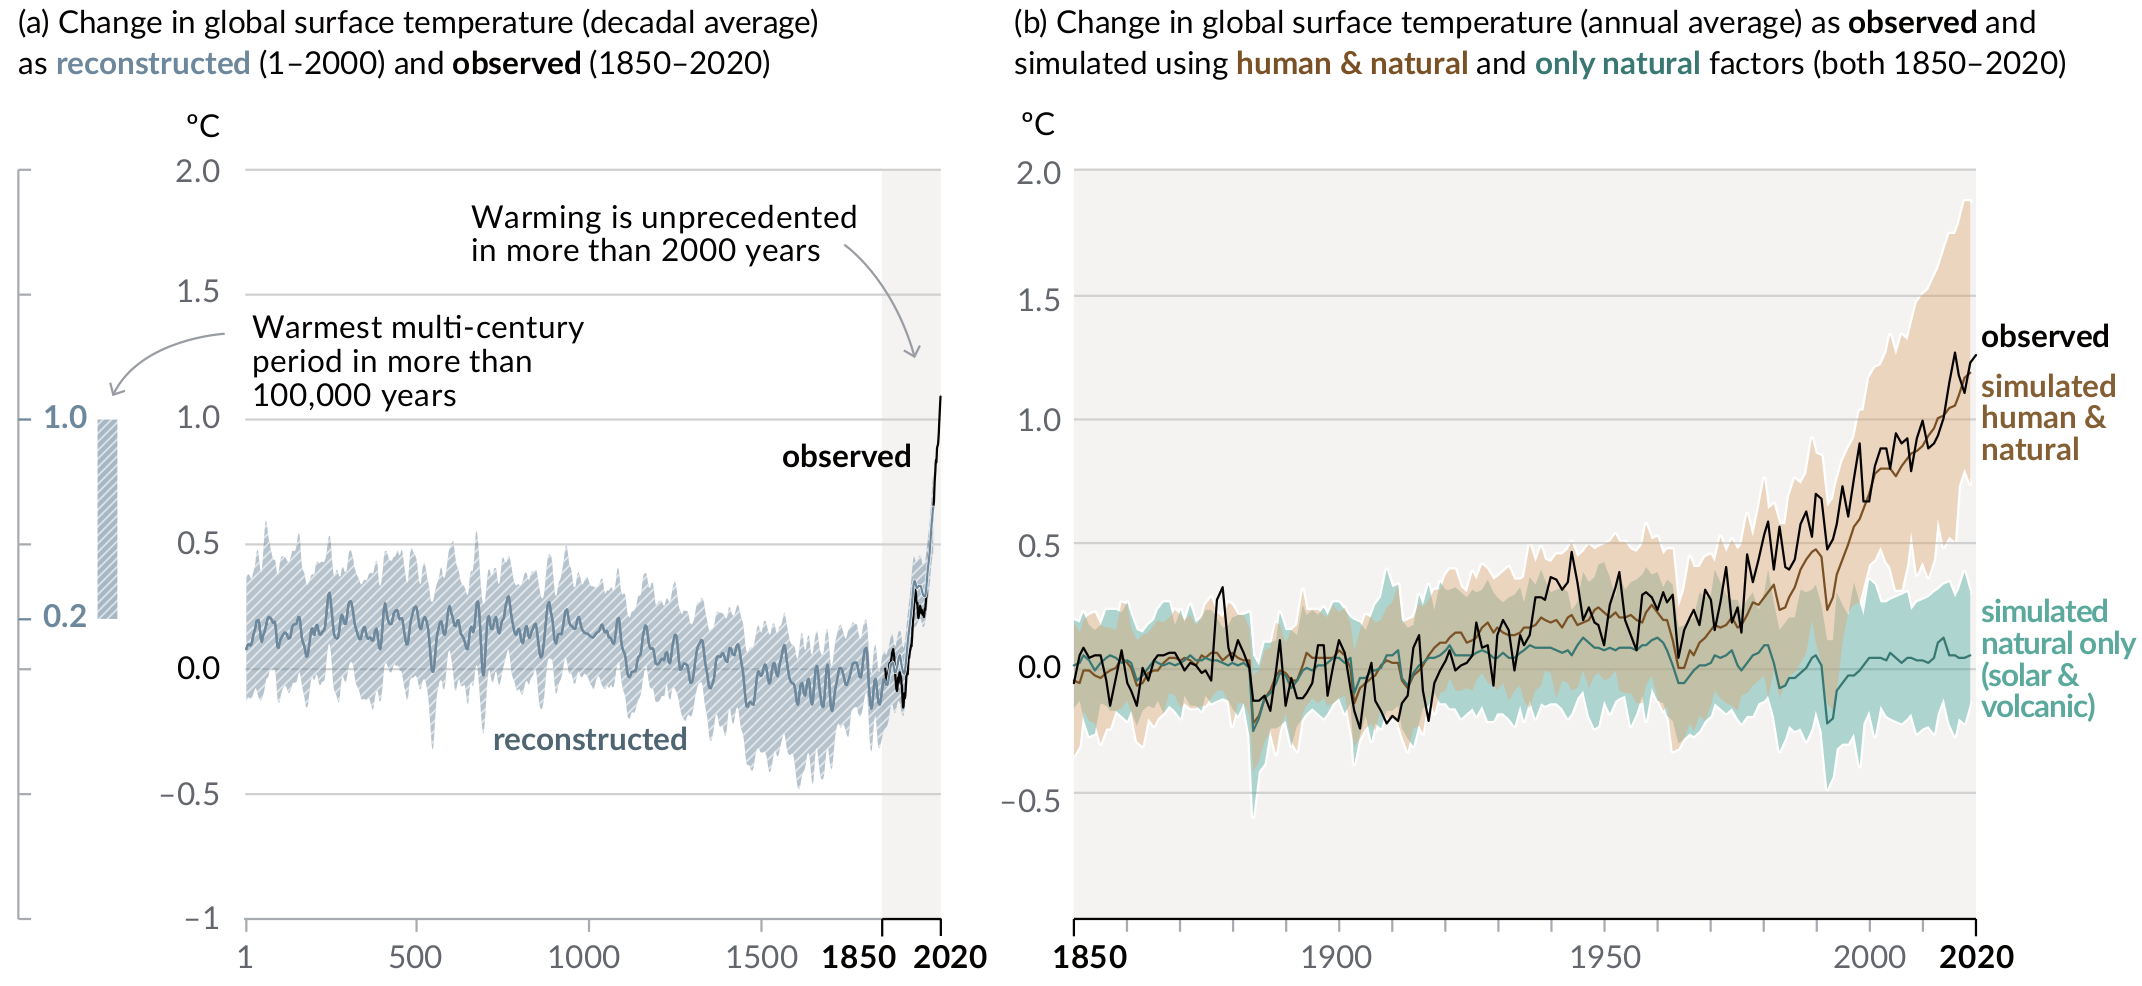
\includegraphics[width=1.0\textwidth]{plots/WG1_temperature.png}
      \end{center}   
    \end{columns}

  \end{scriptsize}
  \end{frame}  


%%%%%%%%%%%%%%%%%%%%%%%%%%%%%%%%%%%%%%%%%%%%%%%%%%%%%%%%%%%%%%%%%%%%%%%%%%%%%%%%%%
\begin{frame}
  \frametitle{\centerline{\hhref{https://www.ipcc.ch/report/ar6/wg1/downloads/report/IPCC_AR6_WGI_SPM_final.pdf}{IPCC Physical Science Basis:} Five illustrative scenarios for future CO$_2$ emissions}}
  \begin{scriptsize}

    \begin{columns}
      \column{0.4\textwidth}
      \begin{itemize}\setlength\itemsep{2.0ex}        
        \item[o] Illustrative scenarios for five possible socio-economic pathways starting in 2015, with their corresponding anthropogenic CO$_2$ and other greenhouse gas (GHG) emissions. They are referred to as the Shared Socio-economic Pathways and they are labelled as SSPx-y, with x ranging from 1 to 5, and y referring to the approximate level of radiative forcing (in watts per square metre).

        \item[o] {\cb SSP3-7.0 and SSP5-8.5} are scenarios with high and very high greenhouse gas emissions that roughly double from current levels by 2100 and 2050, respectively. 
        
        \item[o] {\cb SSP2-4.5} is a scenario with these emissions remaining around current levels until the middle of the century, then starting to decline. 
        
        \item[o] {\cb SSP1-1.9 and SSP1-2.6} are scenarios with very low and low emissions, declining to net zero around 2050, followed by varying levels of net negative CO$_2$ emissions due to anthropogenic removals of CO$_2$.
    \end{itemize}

      \column{0.6\textwidth}
      \begin{center}
          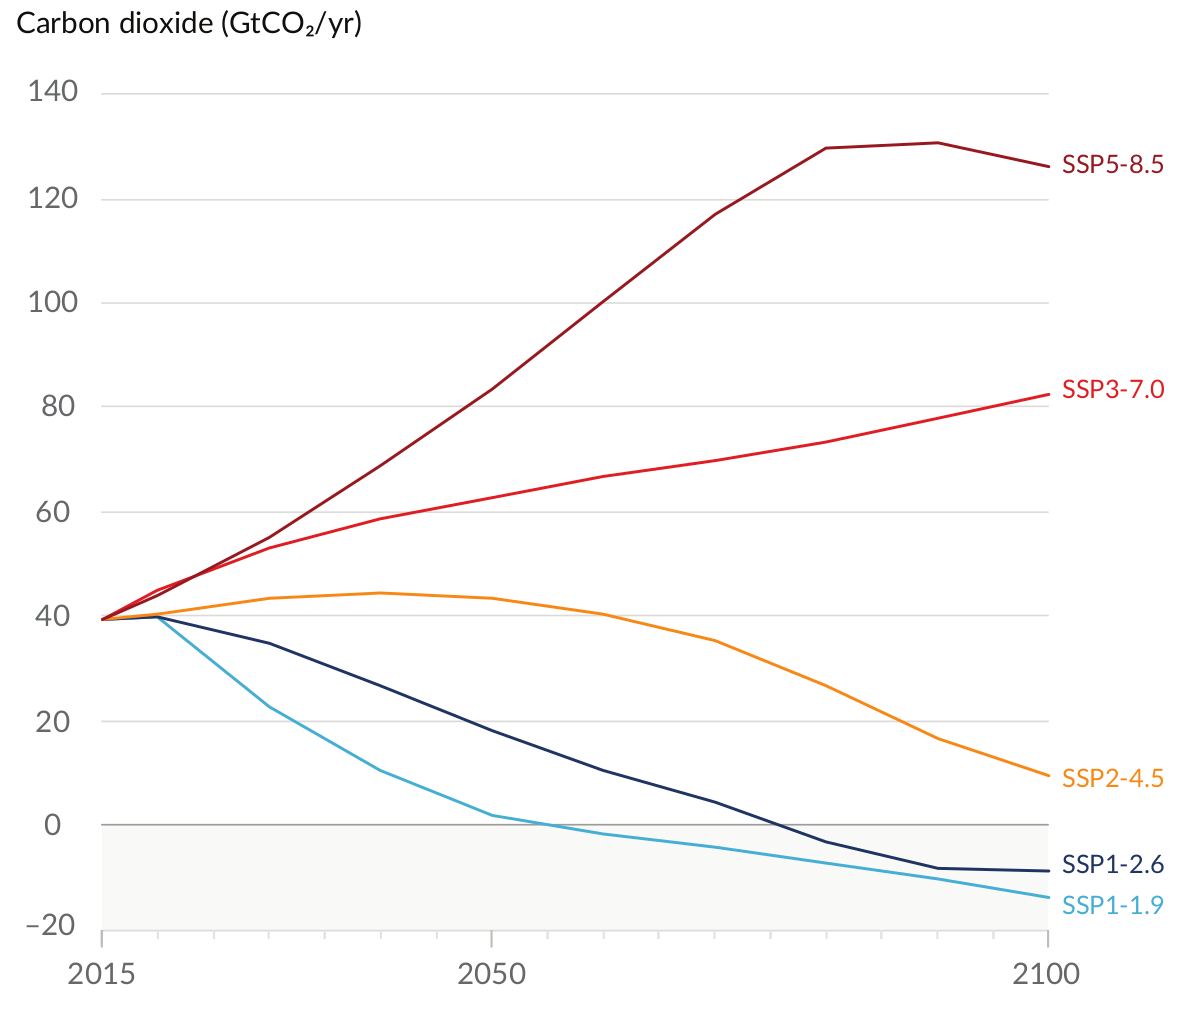
\includegraphics[width=1.0\textwidth]{plots/WG1_co2_scenarios.png}
      \end{center}   
    \end{columns}

  \end{scriptsize}
  \end{frame}

  %%%%%%%%%%%%%%%%%%%%%%%%%%%%%%%%%%%%%%%%%%%%%%%%%%%%%%%%%%%%%%%%%%%%%%%%%%%%%%%%%%
\begin{frame}
  \frametitle{\centerline{\hhref{https://www.ipcc.ch/report/ar6/wg1/downloads/report/IPCC_AR6_WGI_SPM_final.pdf}{IPCC Physical Science Basis:} Predicted temperature for five CO$_2$ scenarios}}
  \begin{scriptsize}

    \begin{columns}
      \column{0.34\textwidth}
      \begin{itemize}\setlength\itemsep{2.9ex}
      \item[o] {\bf Global surface temperature will continue to increase until at least mid-century under all considered emissions scenarios.} 
 
      \item[o] Global warming of 1.5$^\circ$C and 2$^\circ$C will be exceeded during the 21st century, unless deep reductions in CO$_2$ and other greenhouse gas emissions occur in the coming decades.

      \item[o] Extreme weather, rising seas and damaged ecosystems could threaten the safety and livelihoods of billions of people. 

      \item[o] {\it There could be 1.2 billion climate refugees by 2050} - \hhref{https://www.zurich.com/en/media/magazine/2022/there-could-be-1-2-billion-climate-refugees-by-2050-here-s-what-you-need-to-know}{Ecological Threat Register}

      \end{itemize}

      \column{0.7\textwidth}
      \begin{center}
          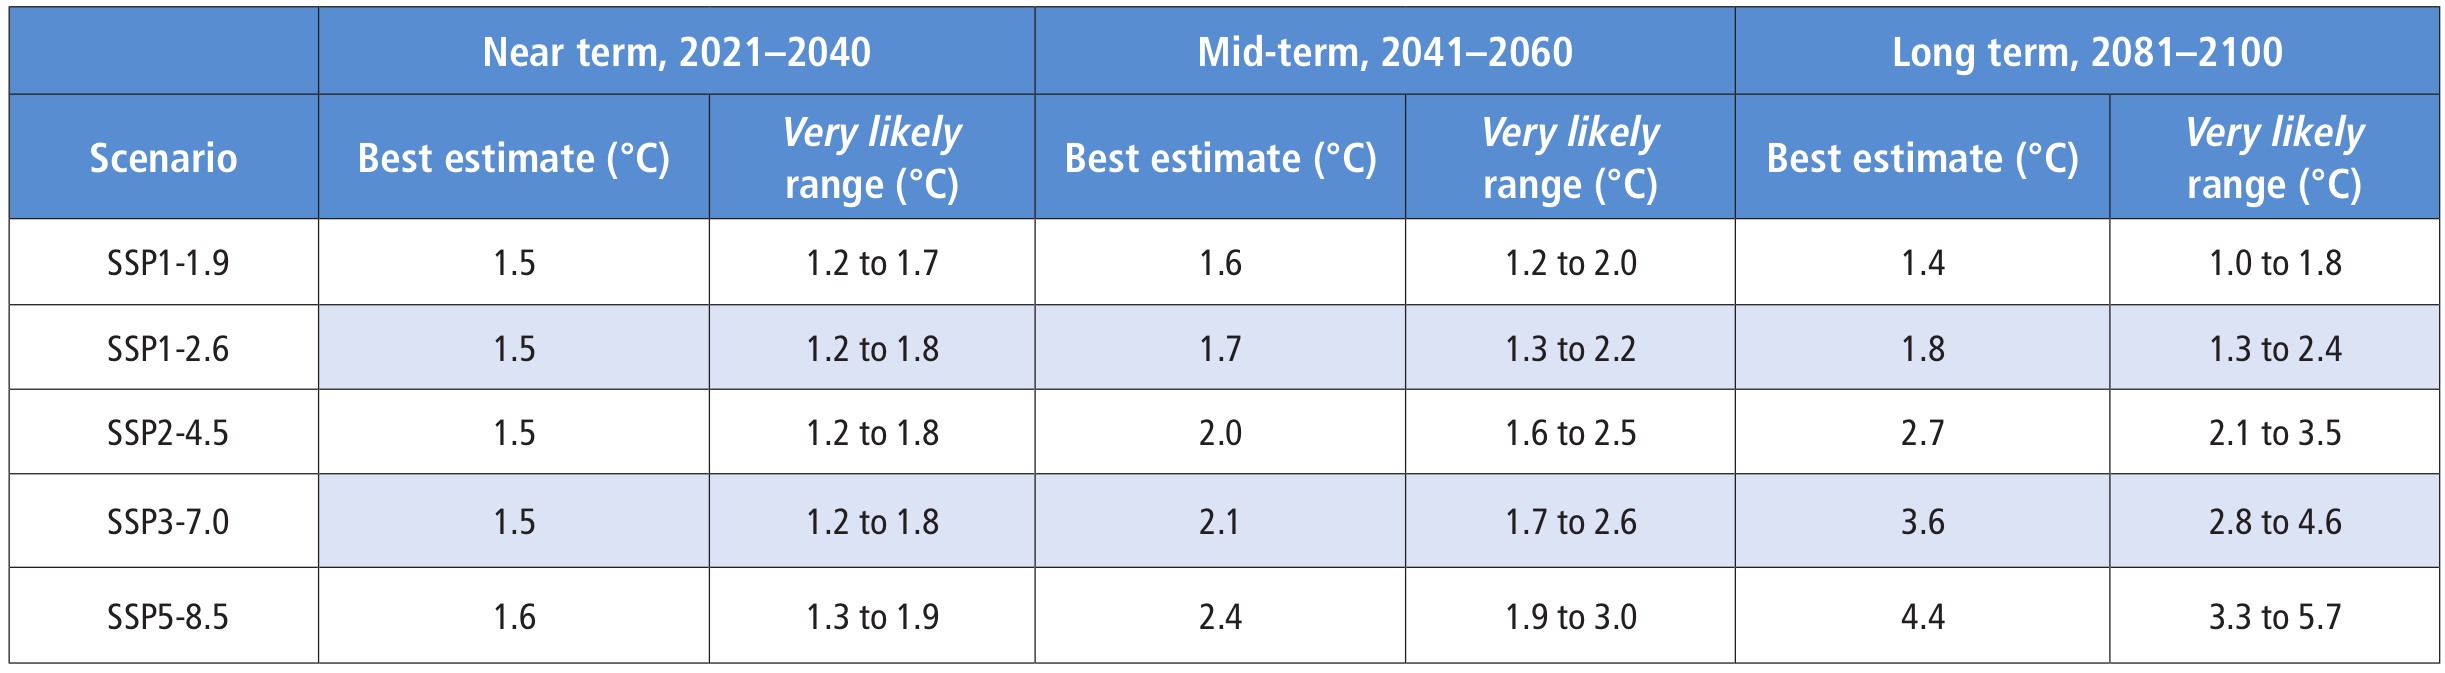
\includegraphics[width=1.0\textwidth]{plots/WG1_predicted_temperature_table.png}\\
          \vspace{0.2cm}
          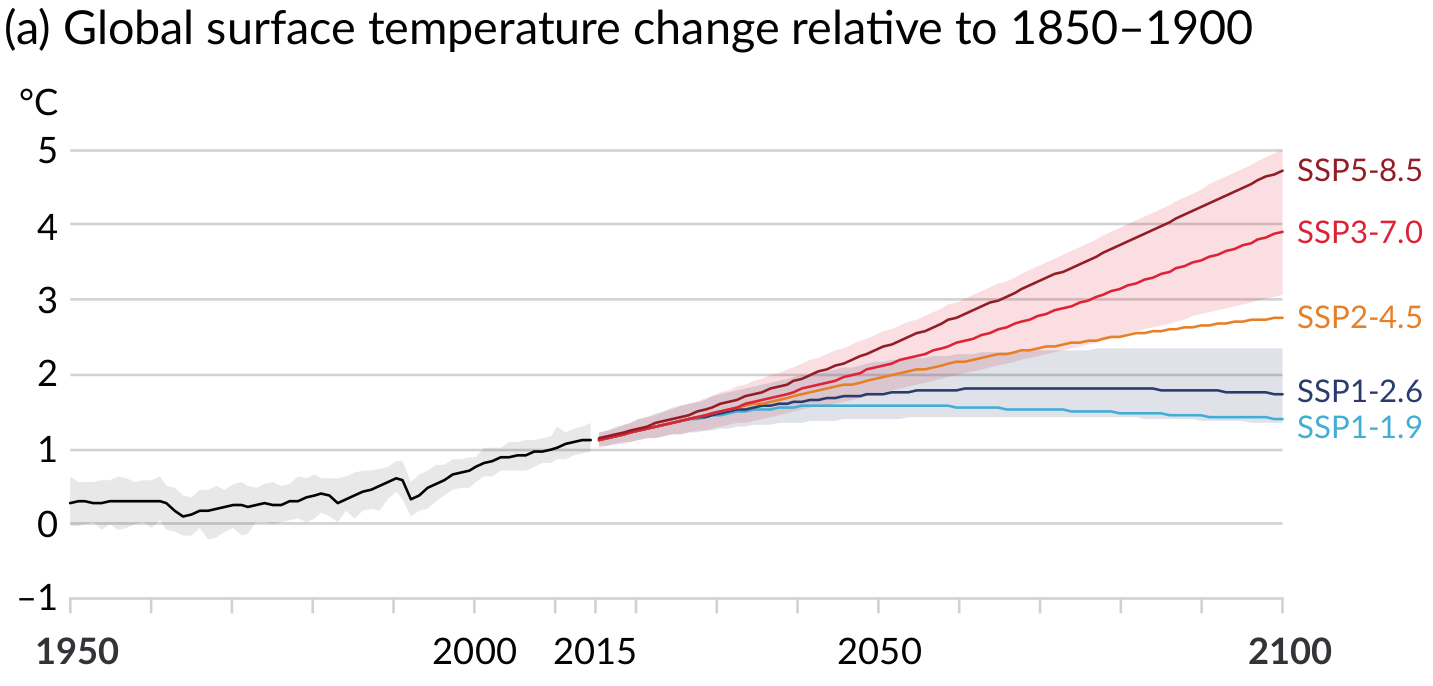
\includegraphics[width=1.0\textwidth]{plots/WG1_SSPs_surface_temperature.png}
      \end{center}   
    \end{columns}

  \end{scriptsize}
  \end{frame}  

%%%%%%%%%%%%%%%%%%%%%%%%%%%%%%%%%%%%%%%%%%%%%%%%%%%%%%%%%%%%%%%%%%%%%%%%%%%%%%%%%%
\begin{frame}
\frametitle{\centerline{\hhref{https://www.ipcc.ch/report/ar6/wg1/downloads/report/IPCC_AR6_WGI_SPM_final.pdf}{IPCC Physical Science Basis:} Predicted surface temperature maps for five CO$_2$ scenarios}}
\begin{scriptsize}

  \begin{columns}

    \column{0.85\textwidth}
    \begin{center}
        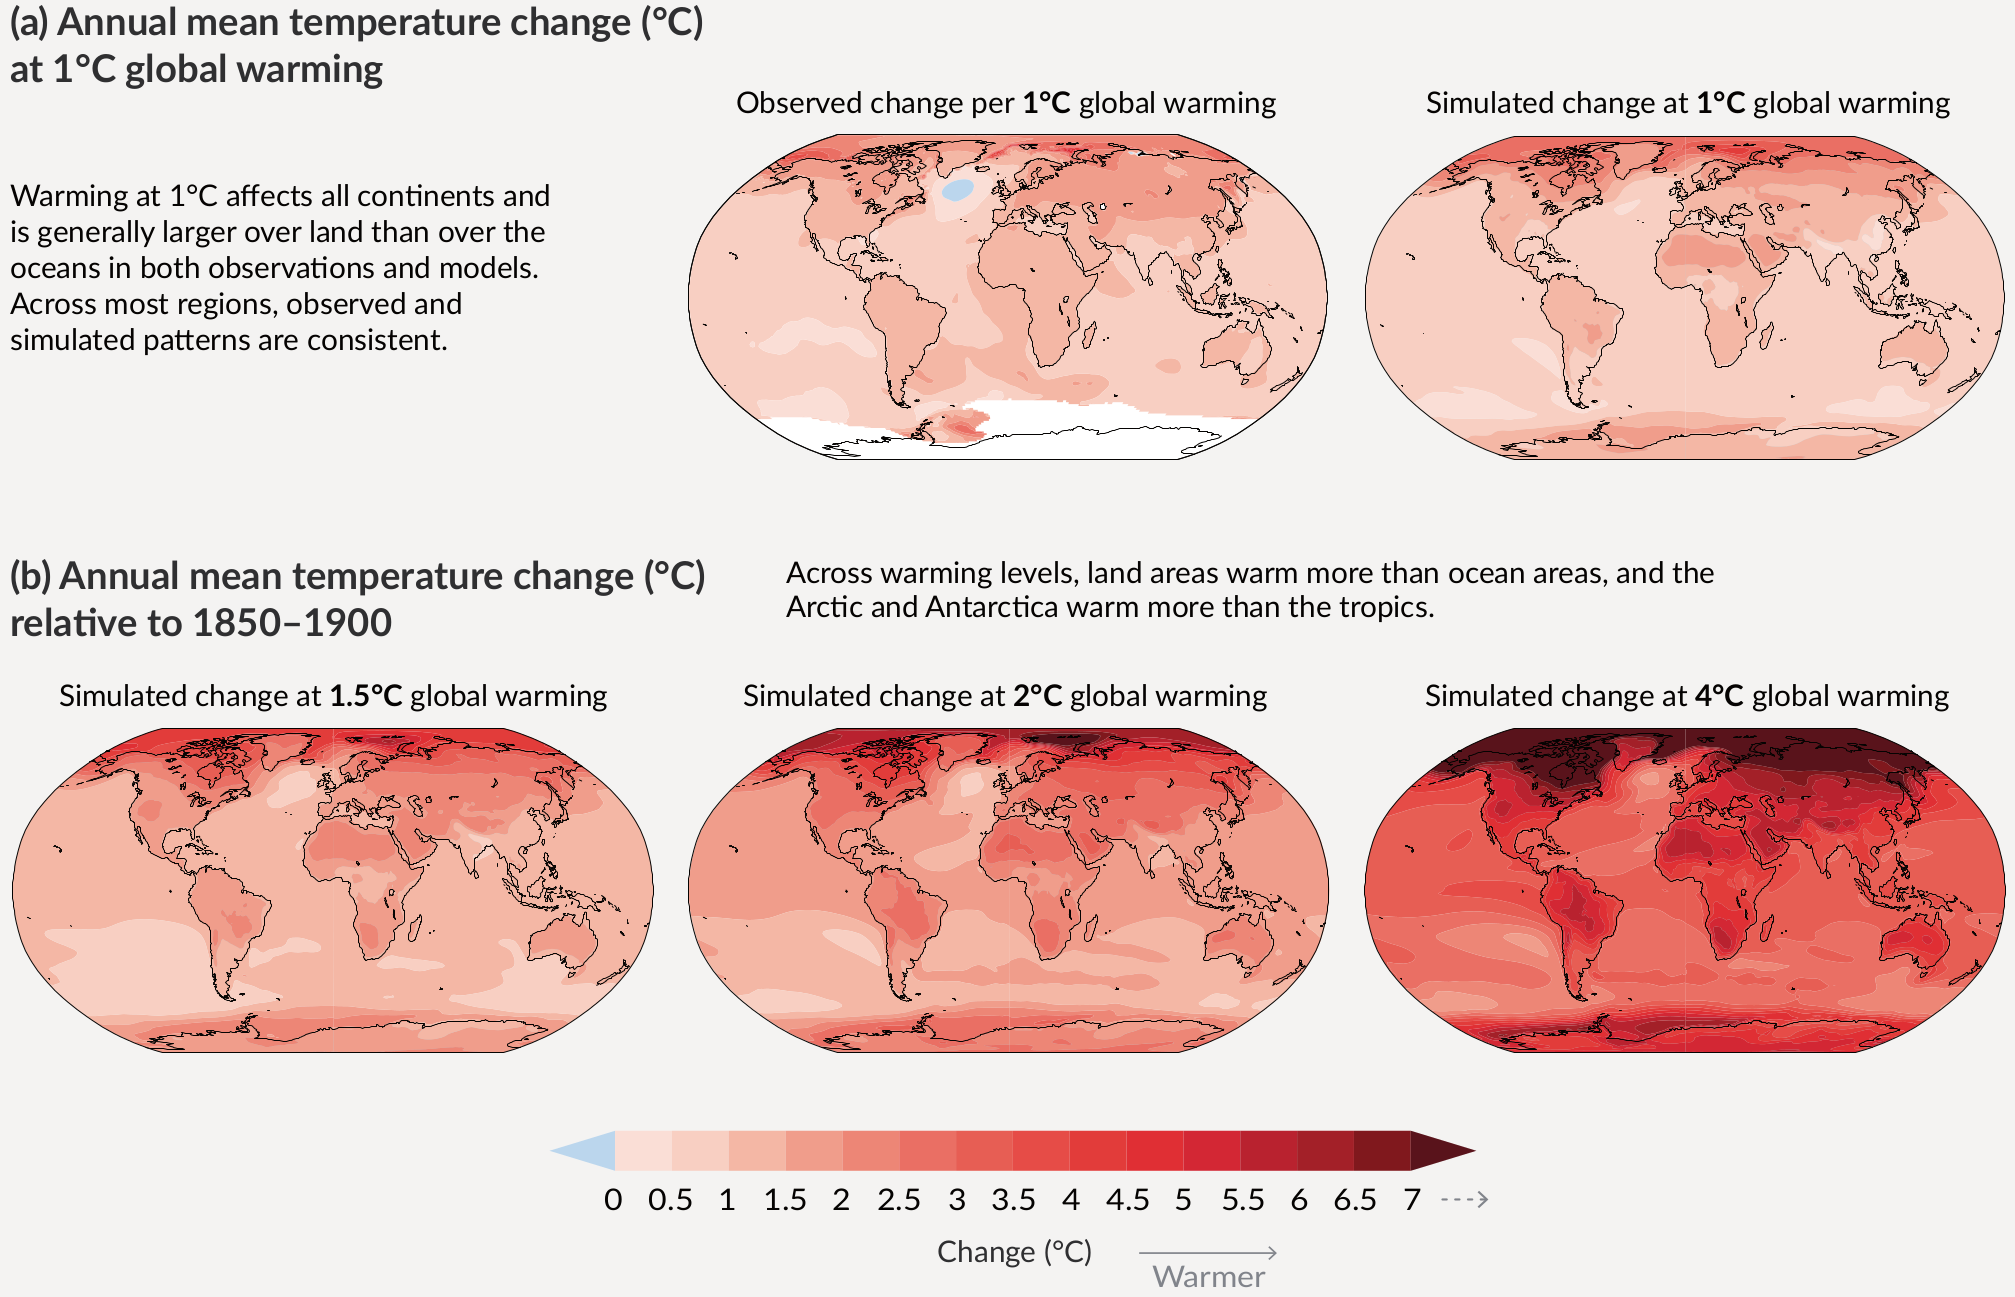
\includegraphics[width=1.0\textwidth]{plots/WG1_SSPs_surface_temperature_maps}
    \end{center}   
  \end{columns}

\end{scriptsize}
\end{frame}  


  %%%%%%%%%%%%%%%%%%%%%%%%%%%%%%%%%%%%%%%%%%%%%%%%%%%%%%%%%%%%%%%%%%%%%%%%%%%%%%%%%%
  \begin{frame}
    \frametitle{\centerline{\hhref{https://www.ipcc.ch/report/ar6/wg1/downloads/report/IPCC_AR6_WGI_SPM_final.pdf}{IPCC Physical Science Basis:} Predicted sea ice melting and sea level raise}}
    \begin{scriptsize}
  
      \begin{columns}
        \column{1.0\textwidth}
        \begin{itemize}\setlength\itemsep{1.9ex}        
          \item[o] {\cb Left:} Past greenhouse gas and CO$_2$ emissions since 1750 have committed the global ocean to future warming (high confidence). Mountain and polar glaciers are committed to continue to melt for decades or centuries (very high confidence). {\it Loss of permafrost carbon following permafrost thaw is irreversible at centennial time scales (high confidence).} Continued ice loss over the 21st century is virtually certain for the Greenland ice sheet and likely for the Antarctic ice sheet. 
  
          \item[o] {\cb Right:} It is virtually certain that global mean sea level will continue to rise over the 21st century. Relative to 1995-2014, the likely global mean sea level rise by 2100 is 0.28-0.55~meter even under the very low GHG emissions scenario (SSP1-1.9), and is 0.32-0.62~meter under the low GHG emissions scenario (SSP1-2.6). Global mean sea level rise of about 2~meter by 2100 and 5~meter by 2150 under a very high GHG emissions scenario (SSP5-8.5) (low confidence) cannot be ruled out due to deep uncertainty in ice-sheet processes.
      \end{itemize}
  
      \end{columns}

      \begin{columns}
        \column{0.5\textwidth}
        \begin{center}
            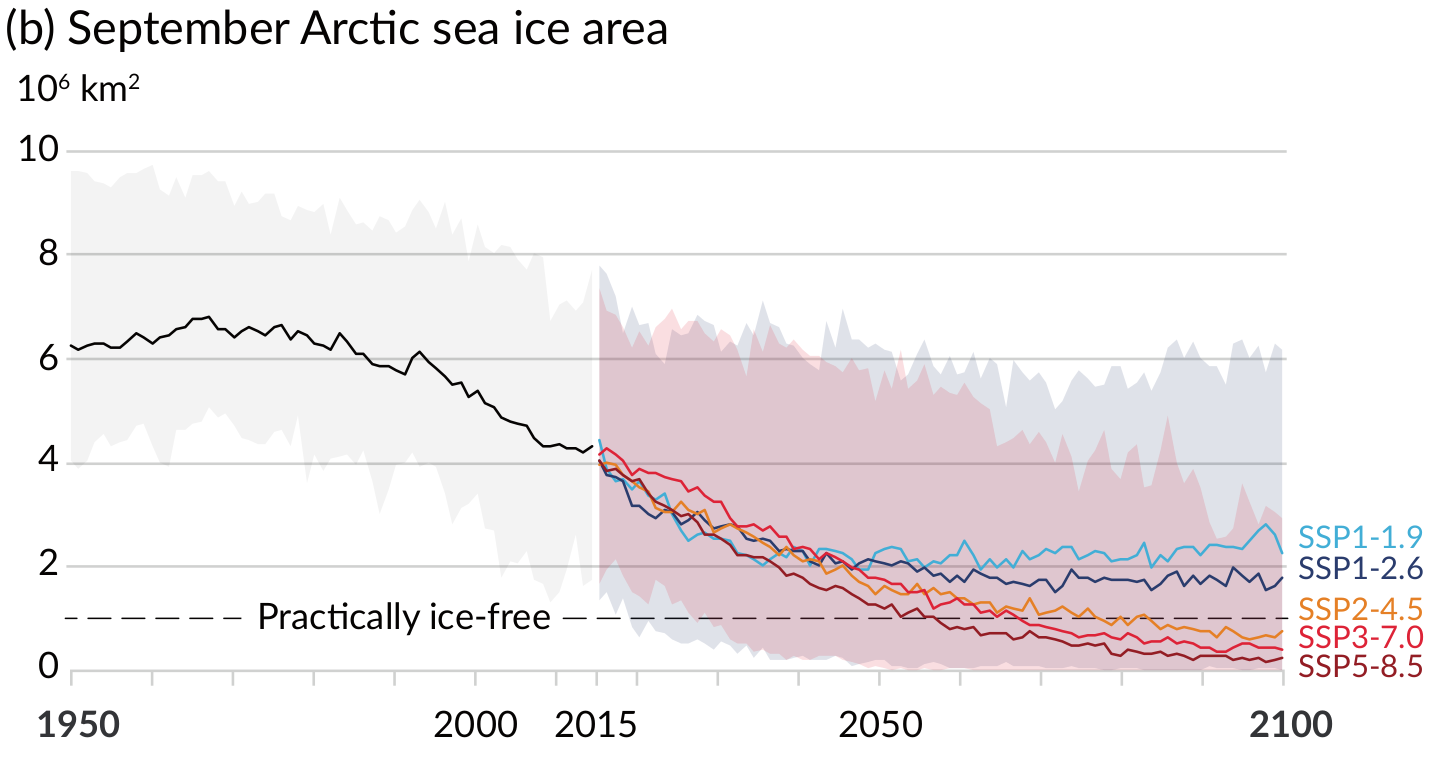
\includegraphics[width=1.0\textwidth]{plots/WG1_SSPs_artic_icearea.png.png}
        \end{center}   

        \column{0.5\textwidth}
        \begin{center}
            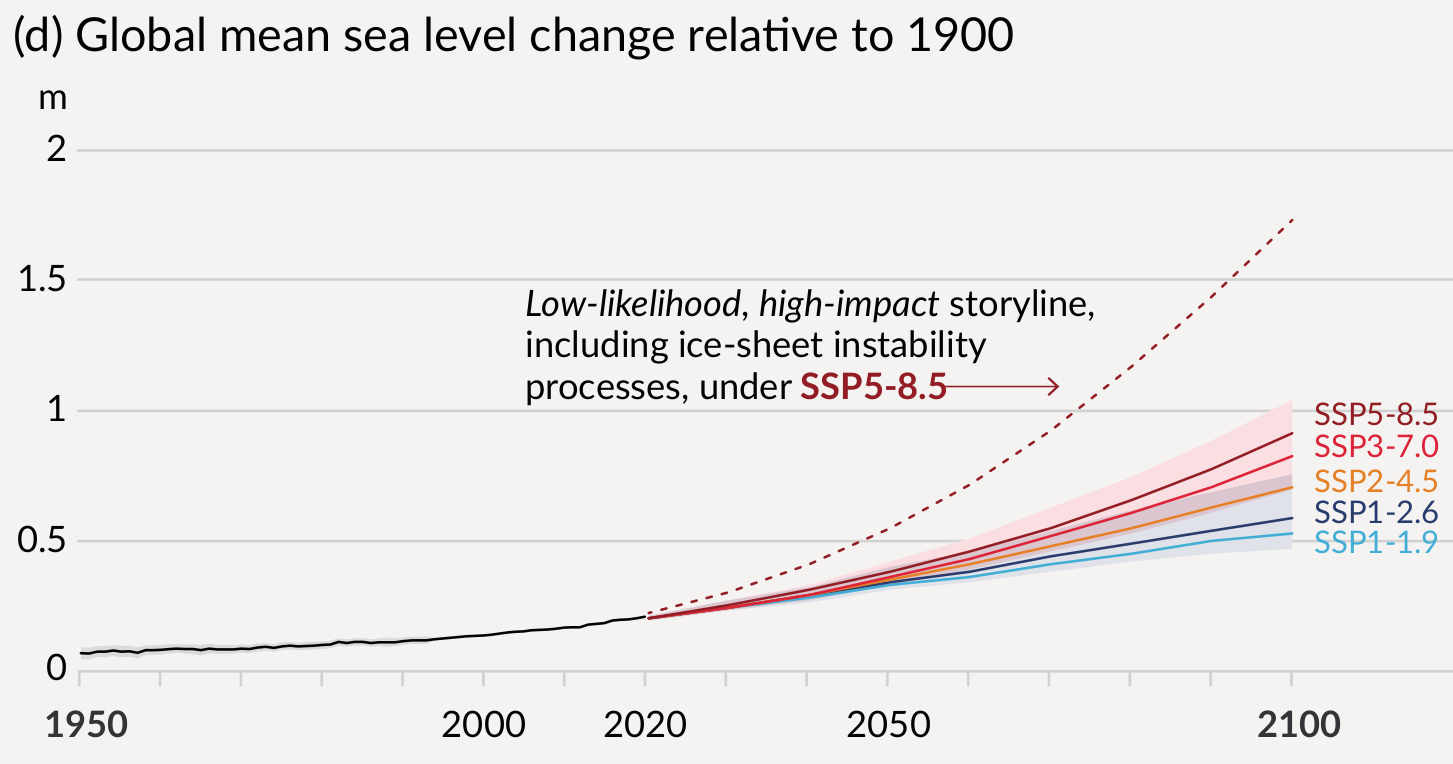
\includegraphics[width=1.0\textwidth]{plots/WG1_SSPs_sea_level_change.png}
        \end{center}   
      \end{columns}
  
    \end{scriptsize}
    \end{frame} 